\subsection{Graphical Interface Interaction}

		A graphical web interface was designed for user friendly
		interaction with TVB . The web interface is accessible locally or
		remotely through a web browser; it can be used by different types of
		users, including those without programming knowledge, and it offers
		good support while the user is learning TVB concepts and workflow
		expectations.  

		\subsubsection{Projects, Accounts, Operations \& Data}

		TVB uses several kinds of entities to model user actions
        and artifacts.

 \begin{figure}[!htbp]

		\centering
		\subfloat[][]{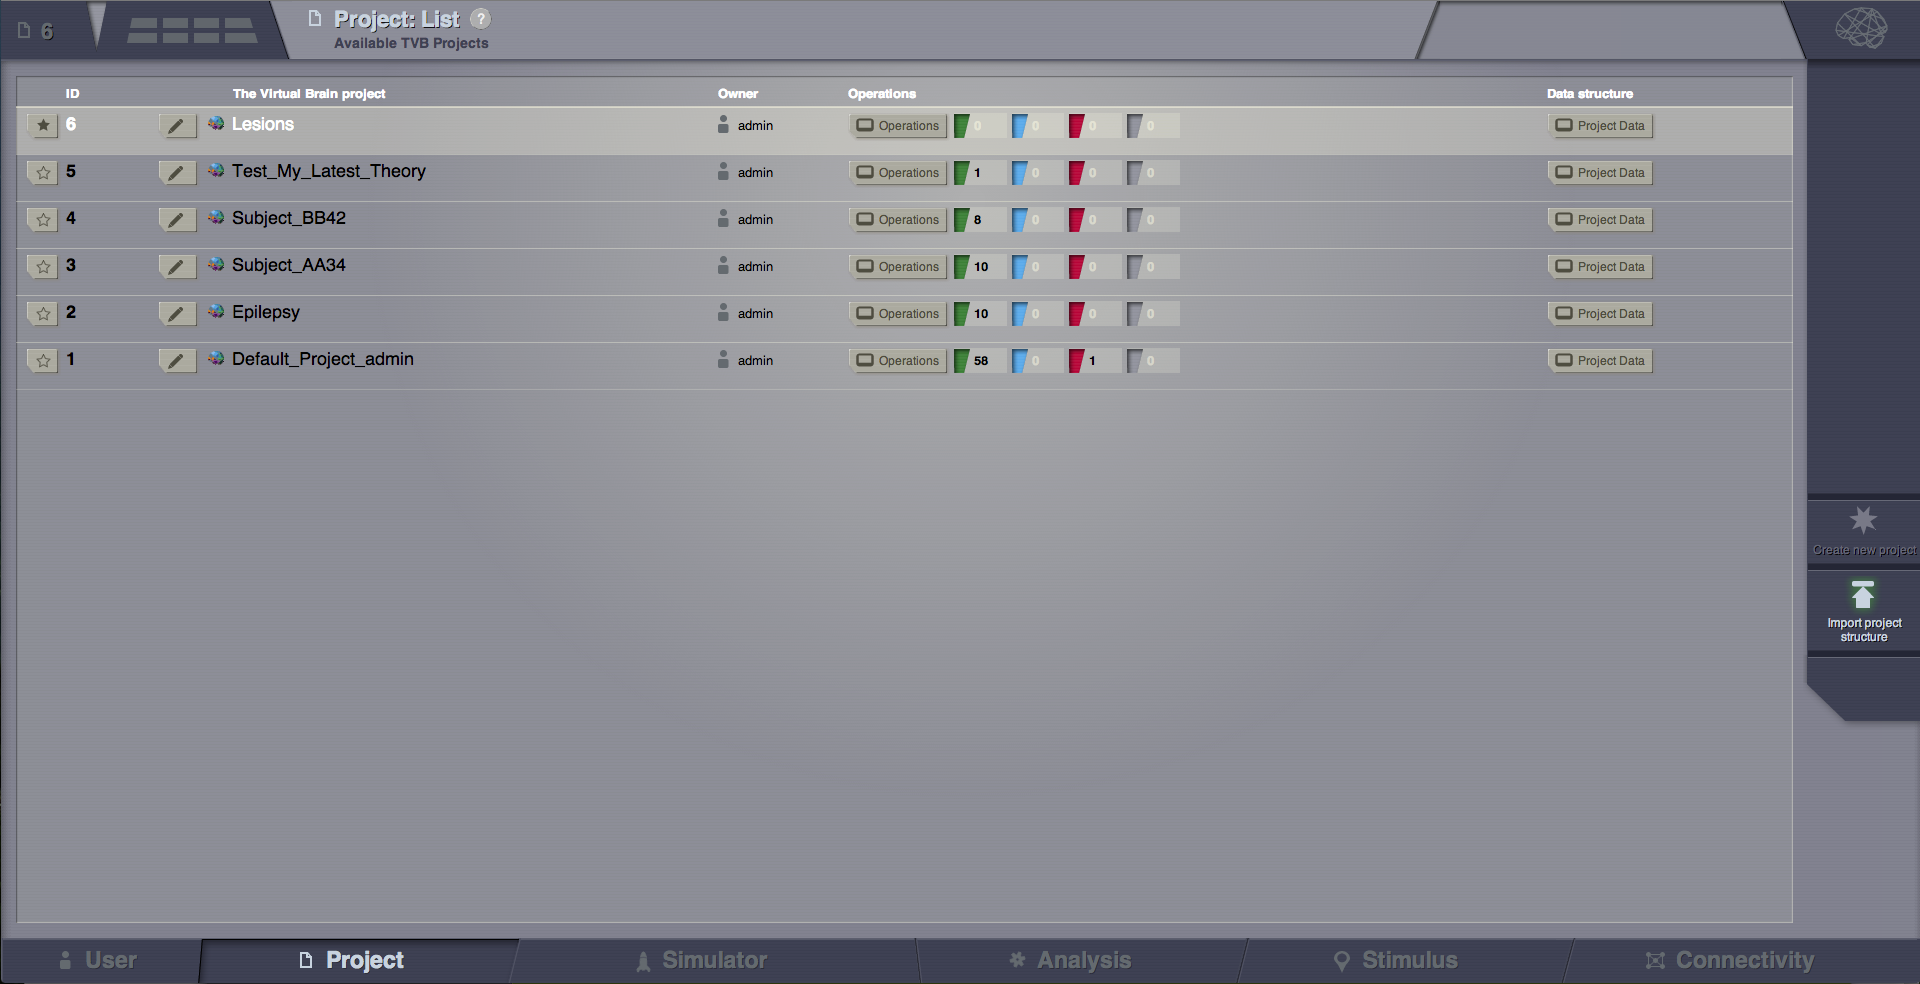
\includegraphics[width=0.47\textwidth]{images/ui_projects.png}}
		\\
		\subfloat[][]{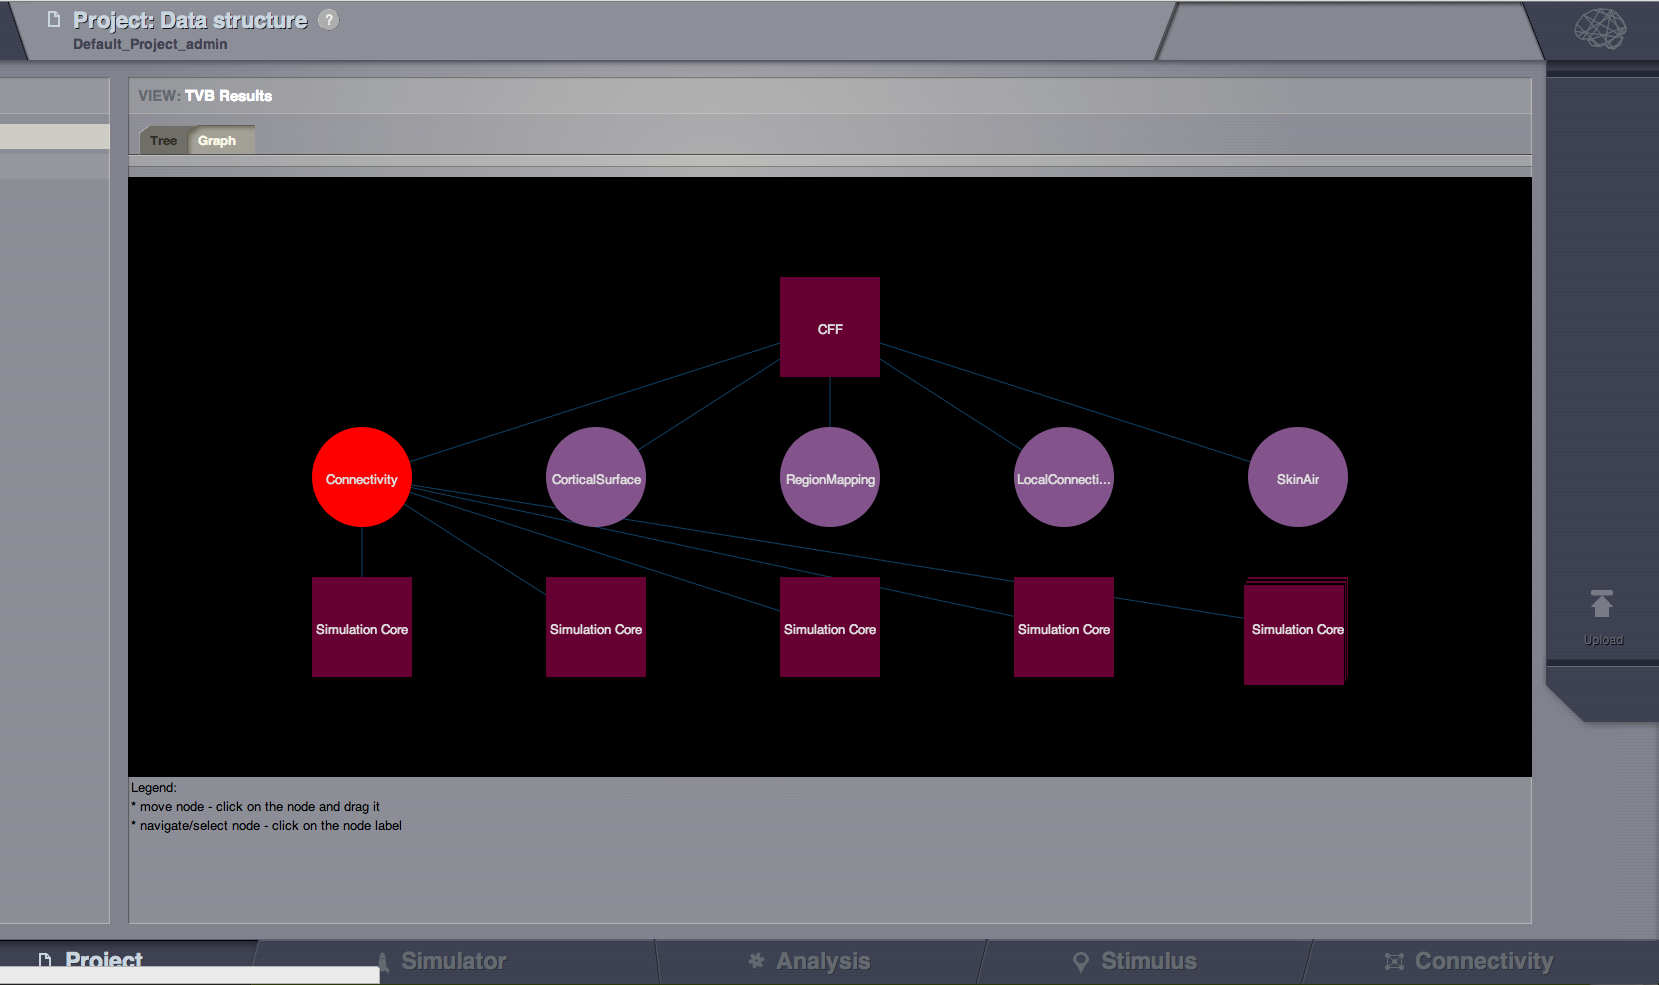
\includegraphics[width=0.47\textwidth]{images/ui_project_graph.png}}
		\\
		\subfloat[][]{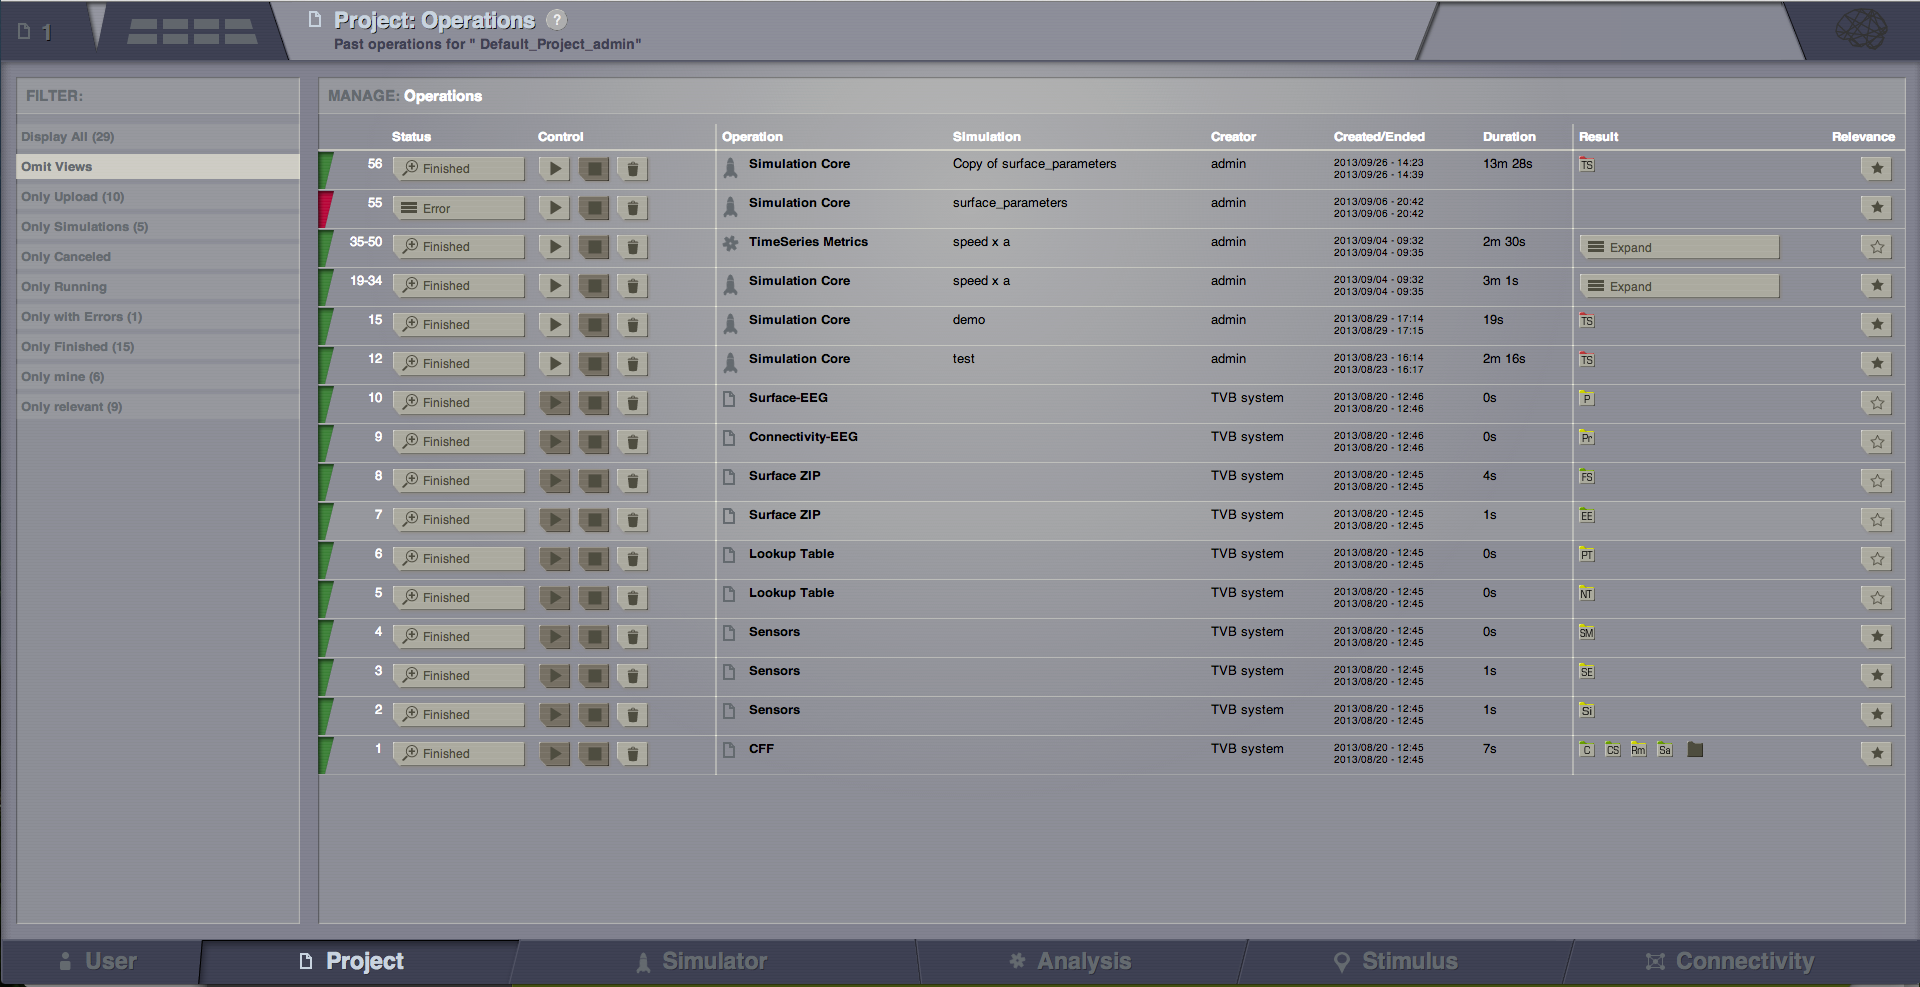
\includegraphics[width=0.47\textwidth]{images/ui_project_operations.png}}
		\\
		\subfloat[][]{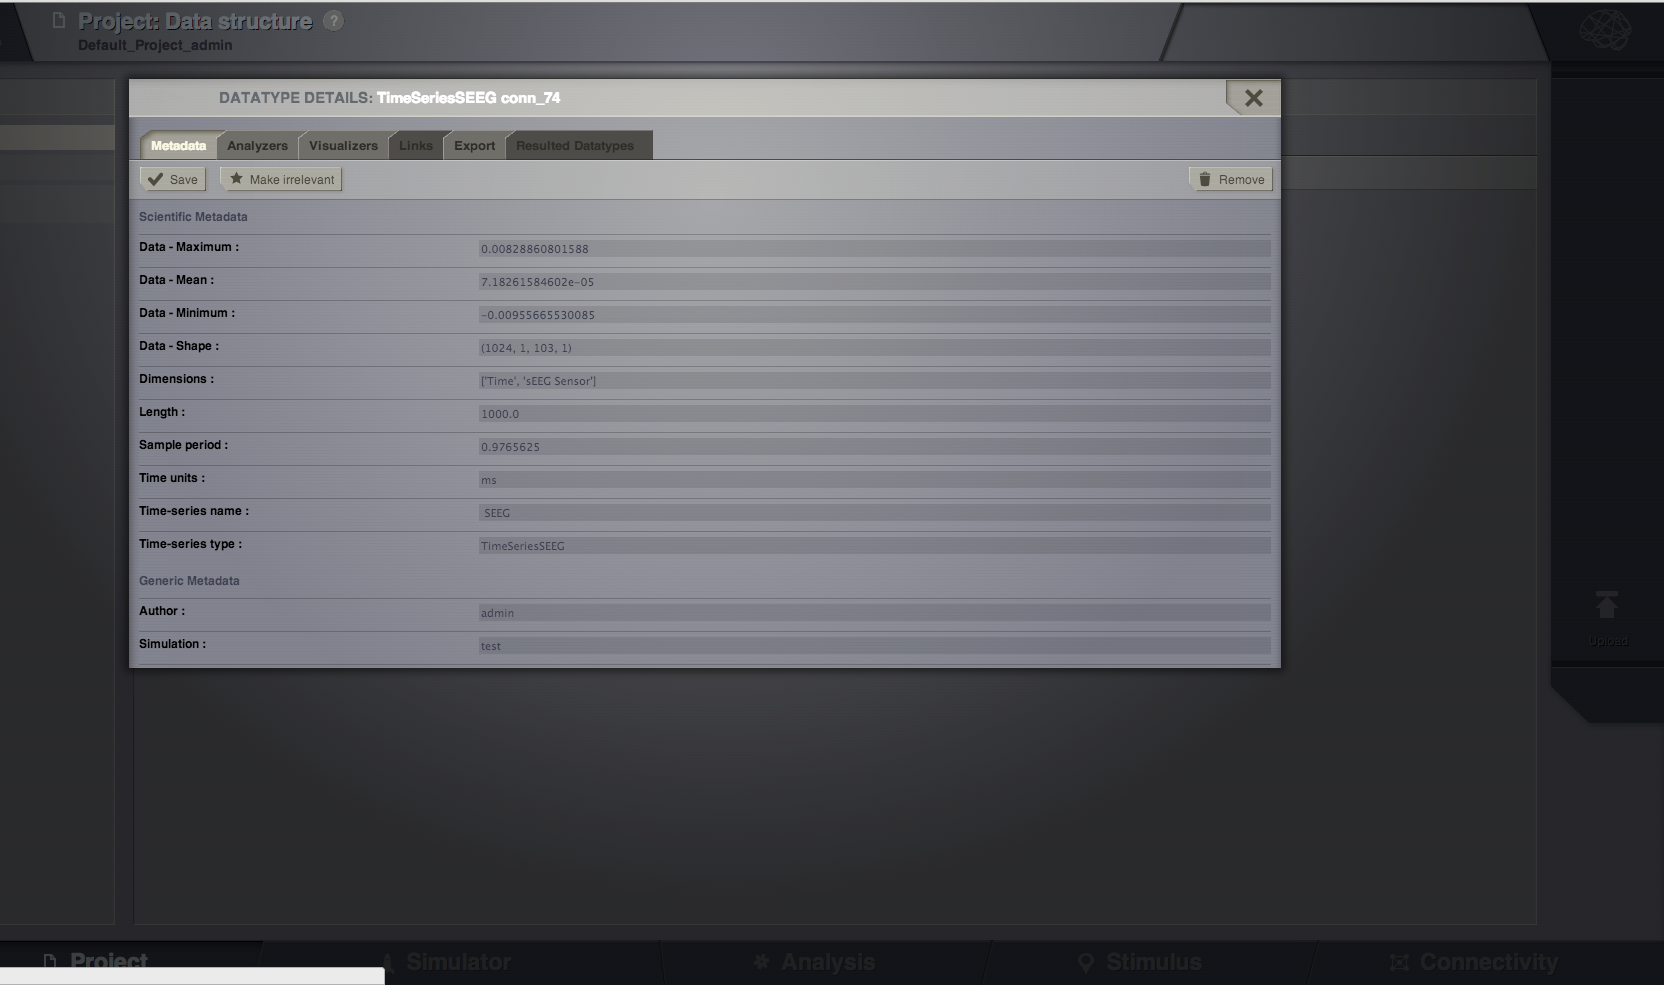
\includegraphics[width=0.47\textwidth]{images/ui_project_datatype_details.png}}
		\caption{\TVB data organization
		(A) View all projects
		(B) 2D graph display of operations with their input and output datatypes 
		(C) View all operations in current project with their status, duration, results, etc
		(D) Datatype details and further available operations for it. This menu becomes available after clicking a datatype result from several places in TVB }
				\label{fig:project}
\end{figure}

		An \emph{Account} or \emph{User} is needed for accessing TVB through
		the web interface.  When TVB web interface is started for the first
		time, the user is requested to provide a username and 
		password for the first account, which acts as an \emph{administrator}.
        Thereafter, others users on the same TVB server can \emph{register}
		for accounts, which are validated by the administrator account.

		A \emph{Project} in TVB is a logical grouping of data and operations: 
        for example, one could choose to
		create a project for each experiment in TVB, while others might
		create projects for each subject of a group. Each project has a single
		user (or account) as owner, but a project may be shared
		with other users to allow for collaboration.

		The execution of an adapter results in an operation, in the
		context of a project. For example, operations are created for each
		simulation, a spectral analysis or surface visualization. 
        Operations have show their status in the user interface, changing from
		\emph{started} to \emph{canceled}, \emph{finished successfully} or
		\emph{finished with error}. 

		A \emph{workflow} in TVB is, conceptually, sequence of operations from simulation,
        through analyses, to visualization(s). A particular workflow applies
		 a default \emph{tag} on the associated operations and
		datatypes.
        The user may also add custom tags to further organize data.

		\subsubsection{Simulator Interface}

		\begin{figure}[!htbp]

		\centering
			\subfloat[][]{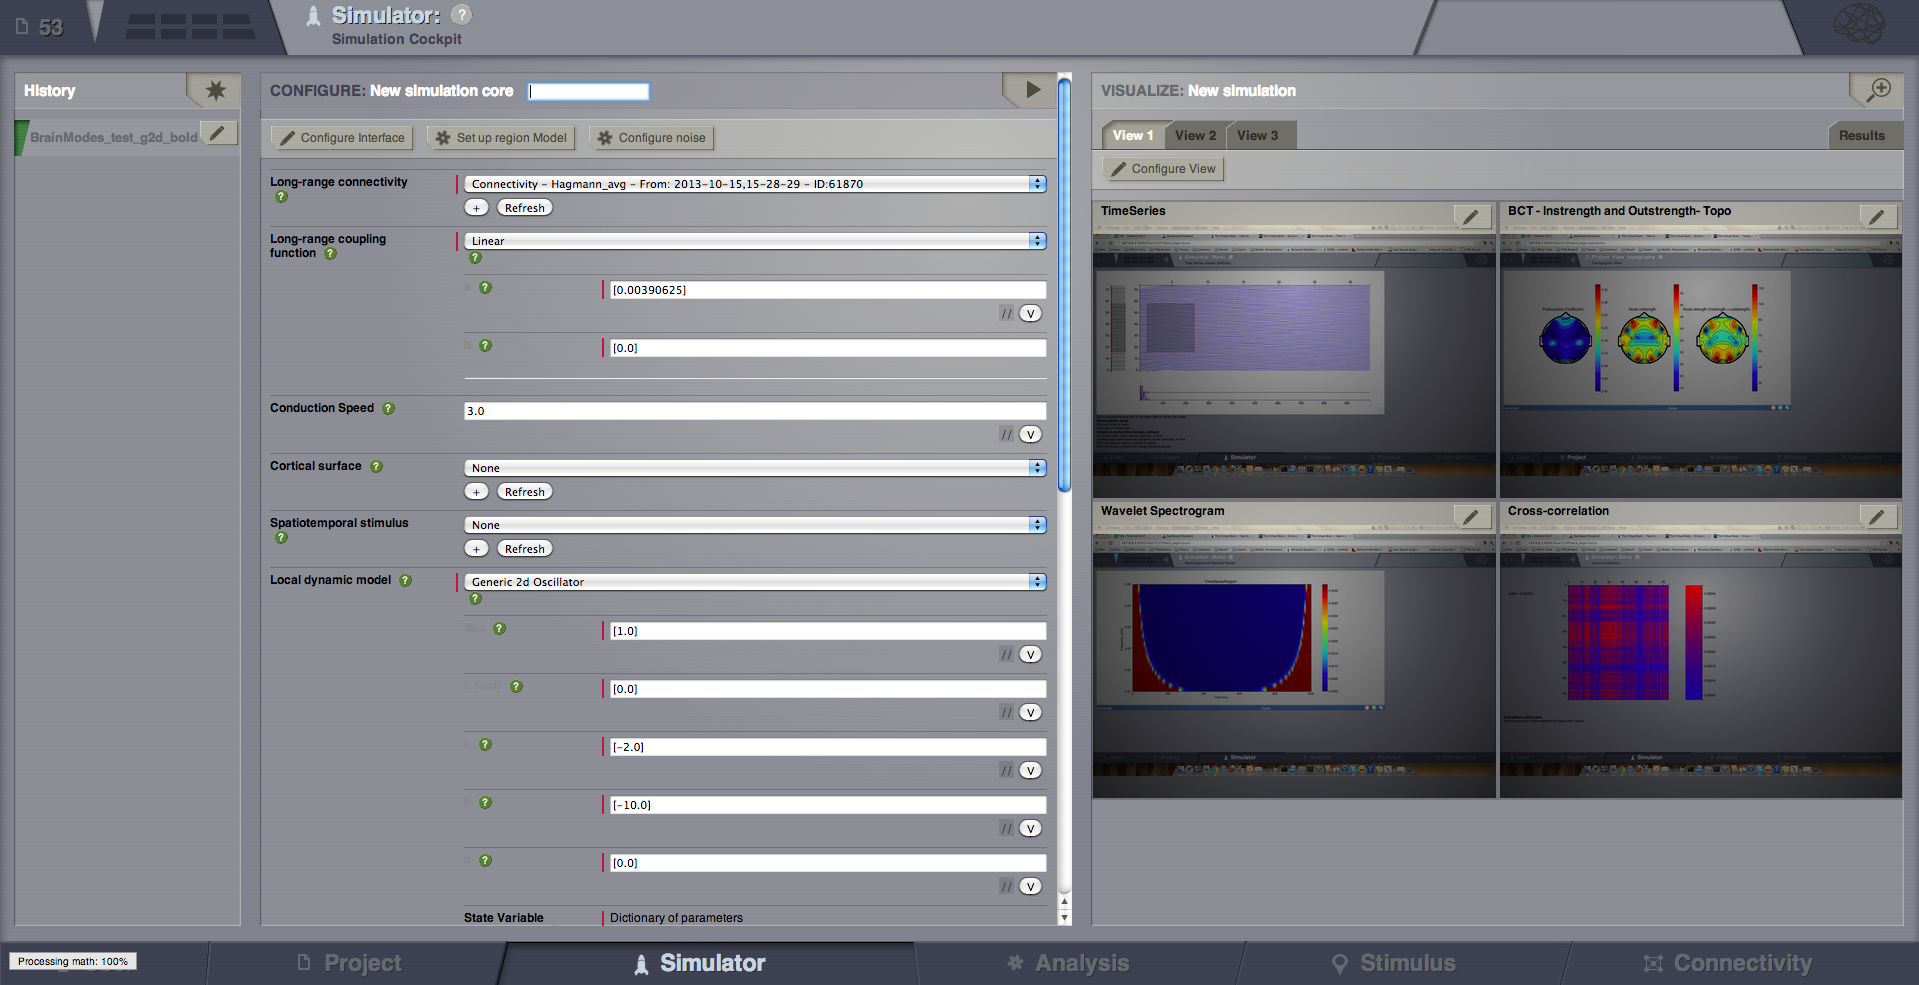
\includegraphics[width=0.47\textwidth]{images/ui_simulator.png}}
			\\
			\subfloat[][]{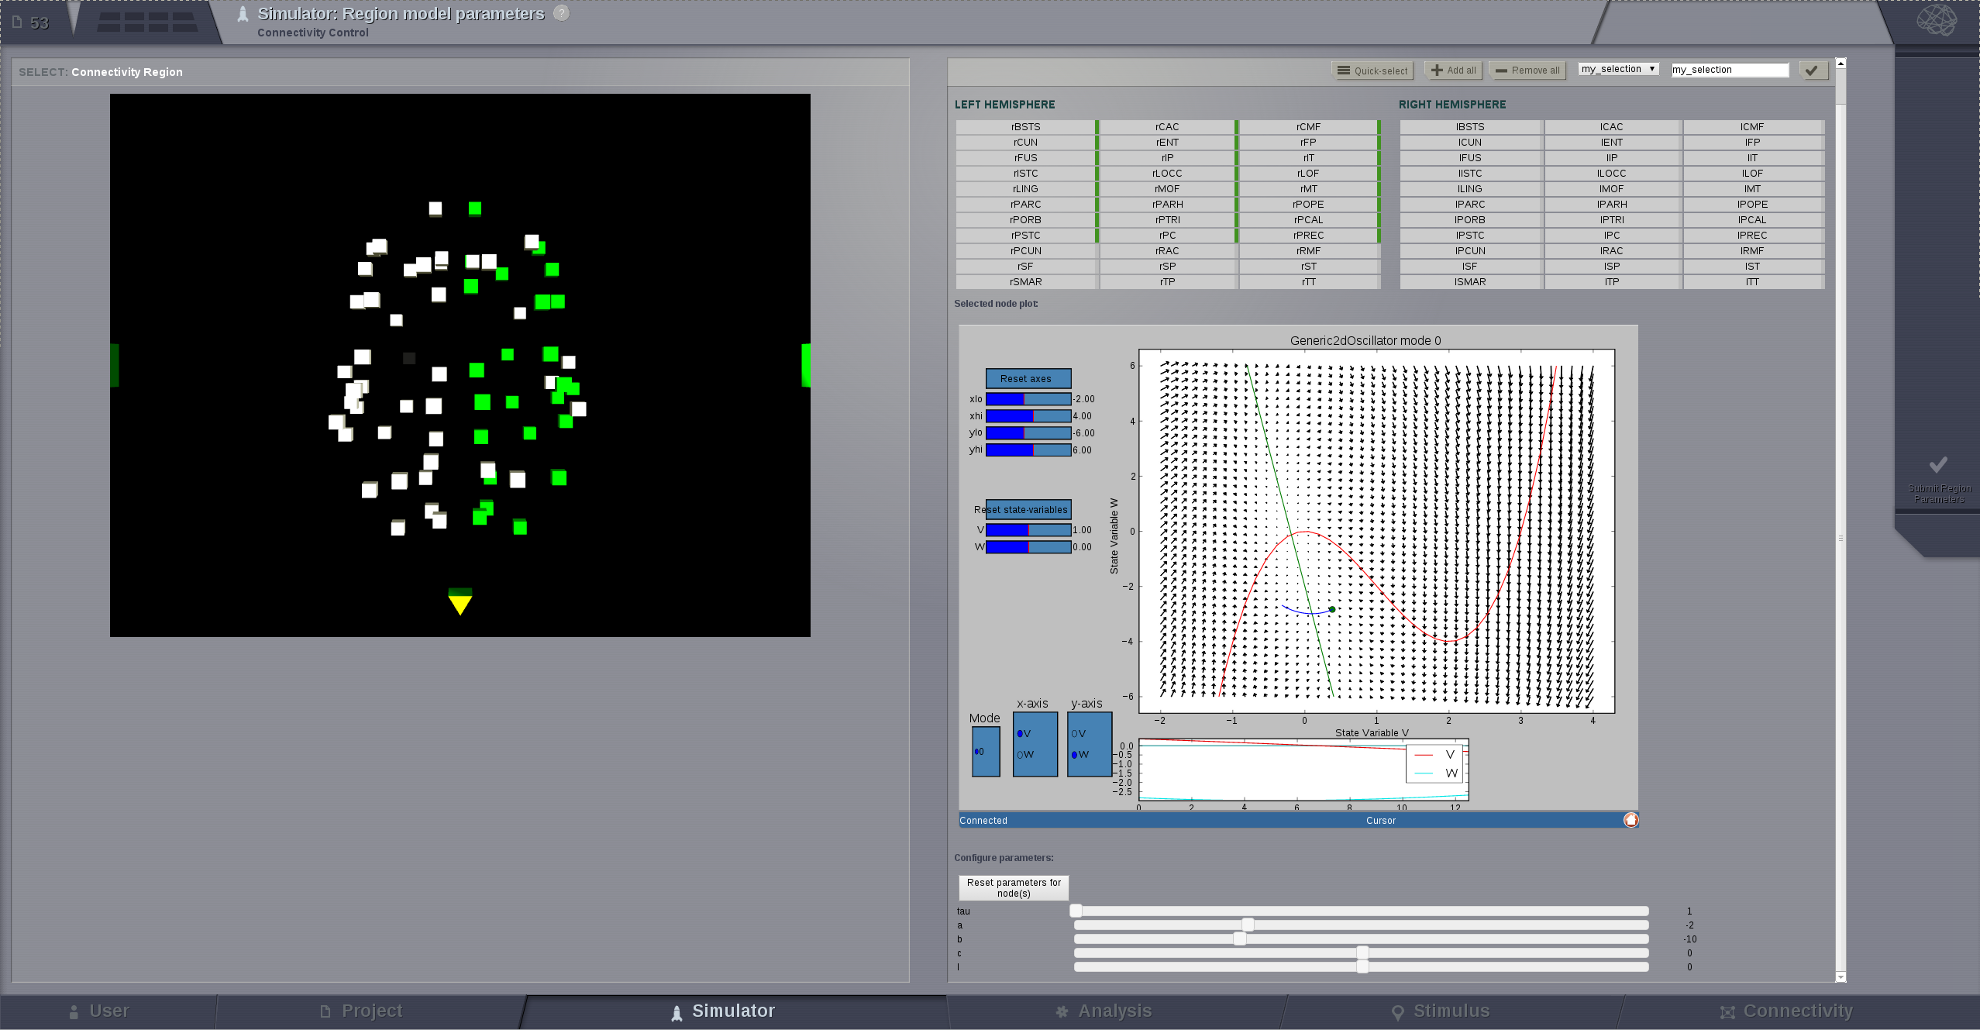
\includegraphics[width=0.47\textwidth]{images/ui_simulator_setup_region.png}}
			\\
			\subfloat[][]{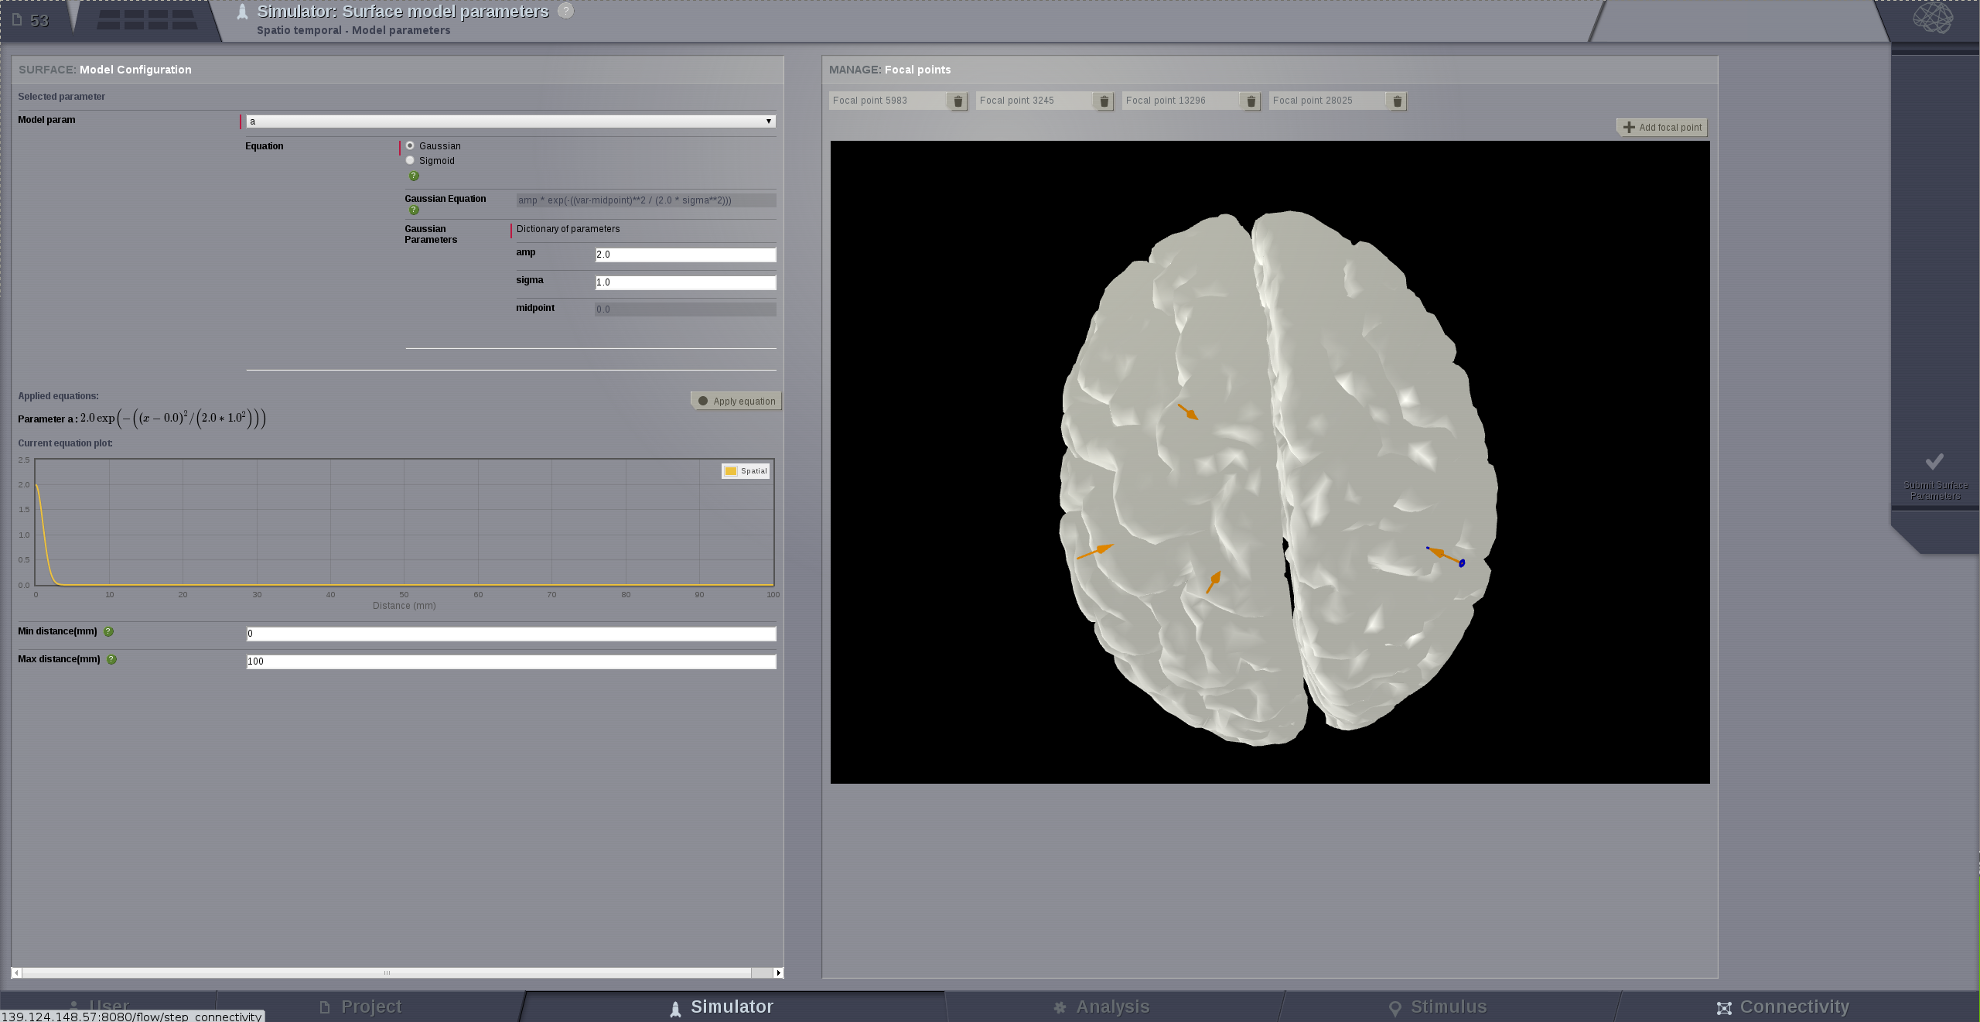
\includegraphics[width=0.47\textwidth]{images/ui_simulator_setup_surface.png}}
			\\
			\subfloat[][]{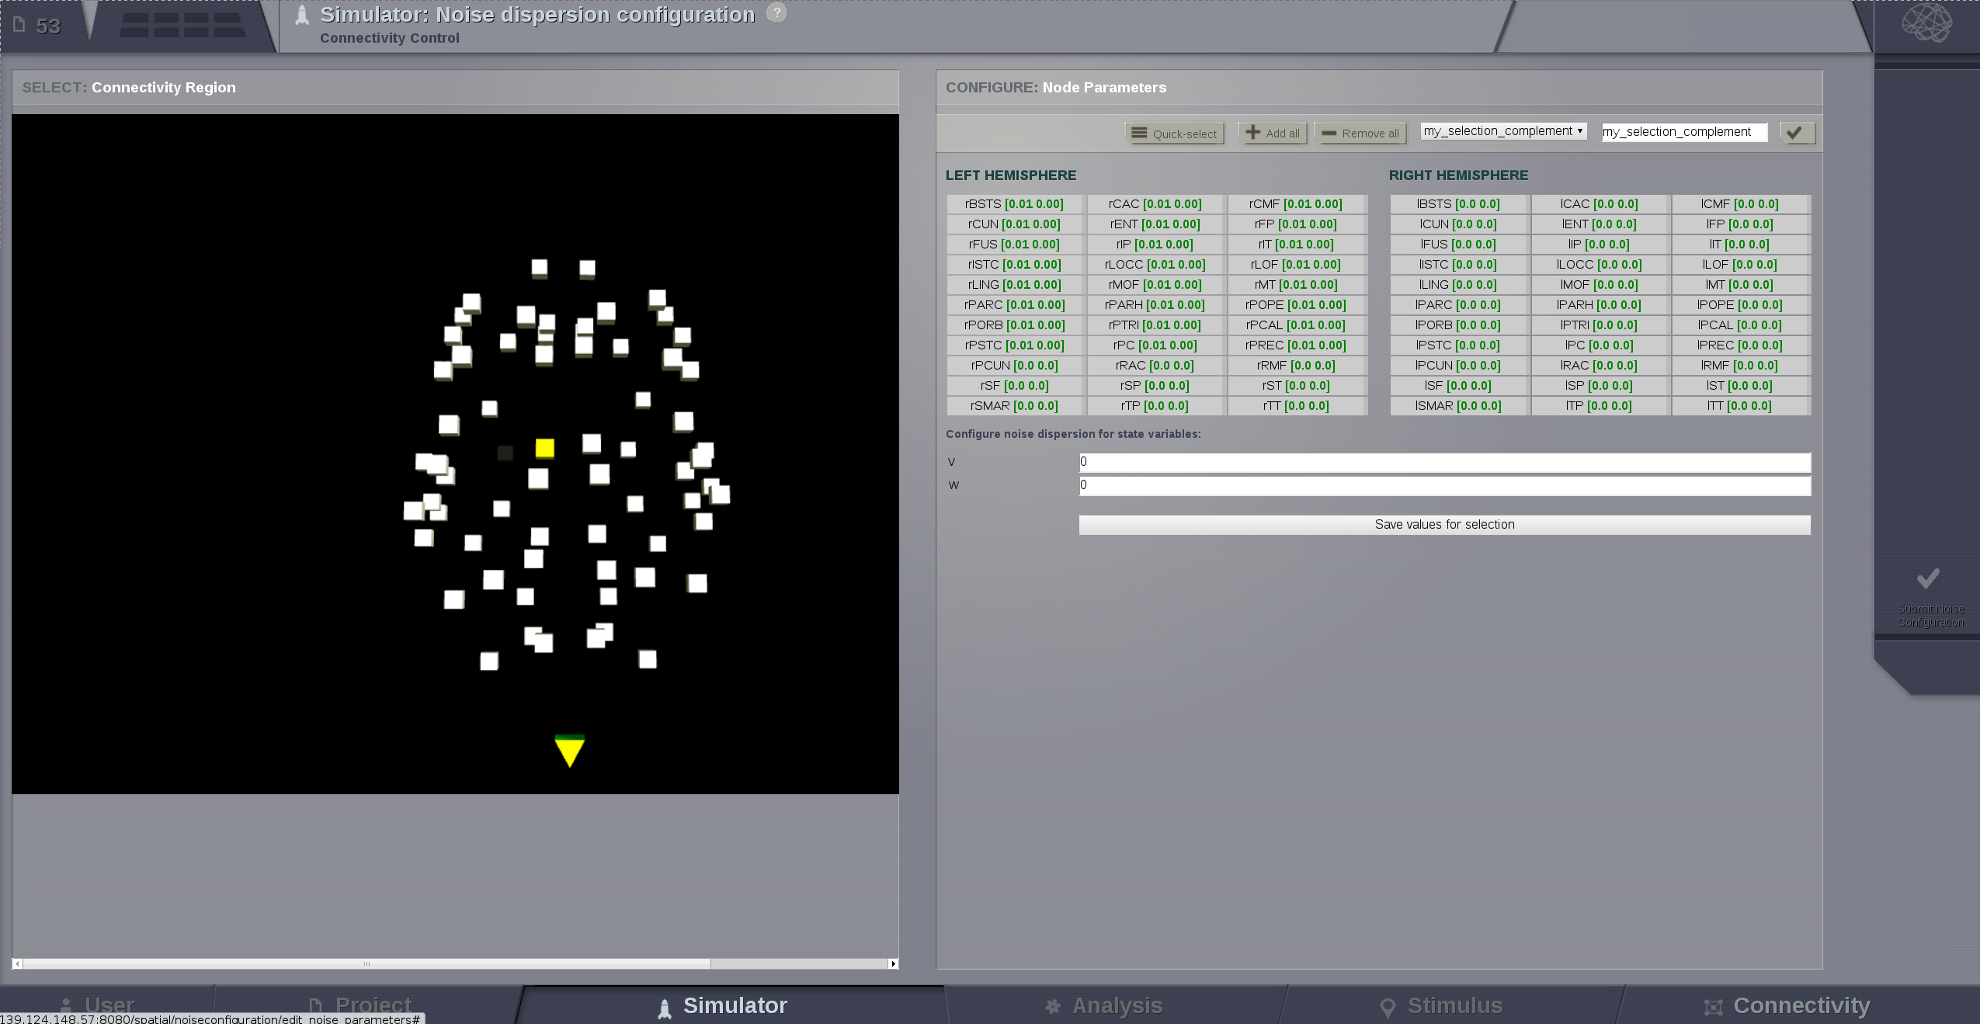
\includegraphics[width=0.47\textwidth]{images/ui_simulator_setup_region_noise.png}}
			\caption{\TVB Simulator Area: 
                (A) View of the main interface. \textit{Left}, the history column displays the
                information about the simulations and their status; \textit{middle}, the
            simulation column is where simulations are configured,
            change of model, parameters, simulation length; \textit{right}, the
            visualization column, provided configurable, multipanel
            visualizers to display the resulting time series or other visualizers
            that will add an analysis step before displaying the results.  (B)
            Region-based simulation configuration. The parameters of the
            mass model can be set independently for each node.  (C) Surface-based
            simulation configuration, allowing the user to define spatially
            inhomogeneous parameters. (D) Define parameters of the simulation's noise. }
		\label{fig:simulator}
		\end{figure}

		The \emph{Simulator} page is a configurable multicolumn interface 
        that combines TVB simulation, analysis and visualization functionalities (Fig.\ref{fig:simulator} A).

		In the left column, a history of all simulations is kept, allowing
        quick access to previous results and their metadata. Here, the user
        may check metadata, add tags and rename or delete the simulation.

		The middle column of the \emph{Simulator} area is where users configure their
		large-scale brain network model. On the top of this column there is a blank
		field to name each particular configuration and a button to launch simulations.
		Via this column, users have access to all the configurable components that might
		be used in a simulation, namely:

		{\small

		\begin{itemize}
			\item long range connectivity (i.e., the connectome or connectivity matrix);
			\item long range coupling function (to scale the weights in the connectivity matrix);
			\item conduction speed;
			\item cortical surface;
			\begin{itemize}
				\item local connectivity kernel;
				\item local connectivity strength (can be configured to be different for each vertex);
				\item region mapping (correspondences between vertices of the surface and anatomical regions in the connectome);
			\end{itemize}
			\item stimulus
			\item local dynamics model (i.e. neural mass model)
				\begin{itemize}
					\item state variable range;
					\item state variables to be recorded and stored;
					\item initial conditions (seed and type of noise used to set random initial conditions);
				\end{itemize}
			\item integration scheme;
			\begin{itemize}
				\item if stochastic, the random seed can be set as well as the type of noise (white, coloured);
				\item integration time step size;
			\item monitors (you can set the monitors period to downsample the raw time-series)
			\item simulation length
			\end{itemize}
		\end{itemize}
		}

		Additional information about the components (e.g., modules, datatypes
		and their attributes) is available  by clicking on the question
		mark icon next to each element. This documentation is pulled from the
		annotations provided by the traits system and documentation strings.

		Specific pages are accessible for setting up the neural mass model
		parameters in region-based and surface-based simulations, as well as
		for configuring the noise amplitude in stochastic integrations (only
		for region-based simulations) (Figs. \ref{fig:simulator} B, C and D)
		The ``Set up region Model'' area consist of an interactive phase-plane
		display. This tool shows the 2-dimensional planes of the general
		N-dimensional phase space of the local dynamic model. This tool is
		used to observe how the dynamics of the physical model change as a
		function of its parameters, acting as a guide to set those parameters
		appropriately.

		On the right column, different displays can be configured to show 
		the simulated time series and to add an analysis step with a subsequent
        visualization of the
		results, for example, computing the correlation coefficients and visualizing the
		resulting matrix).

        For many of the parameters, such as 
        a parameter of the local dynamics model, coupling
		strength, conduction speed, among others, 
        it is possible to specify a range of evenly
        spaced values, and launch the corresponding sweep in
        parallel, using several CPU cores. When the simulation results
        are available, a common metric, such as average variance or 
        degree of synchronization, is applied to the time series, and a 
        one or two dimensional plot, determined by the number of parameters
        for which parameter ranges were provided, is shown, allowing
        the user to see how the simulation changes with the chosen parameters
		(Fig.\ref{fig:visualizers} A).
		
		\subsubsection{Analysis \& Visualizers}

			TVB does not intend to provide fully featured, complex data analysis
            techniques, which have been well covered by other packages. 
            Instead, we offer a minimal set of standard algorithms to quickly
            validate simulation results or compare with imported patient data; 
            these include principal and independent component analyses, 
            Fourier and wavelet spectral analyses, correlation and coherence
            analyses, and for connectivity, an interface to the Brain 
            Connectivity Toolbox \citep{Rubinov_2010}. 

			For each of the datatypes produced in TVB, one or more
			visualizers are available, each taking advantage of the best
            techniques available:

			 \begin{figure}[!htbp]
					\subfloat[][]{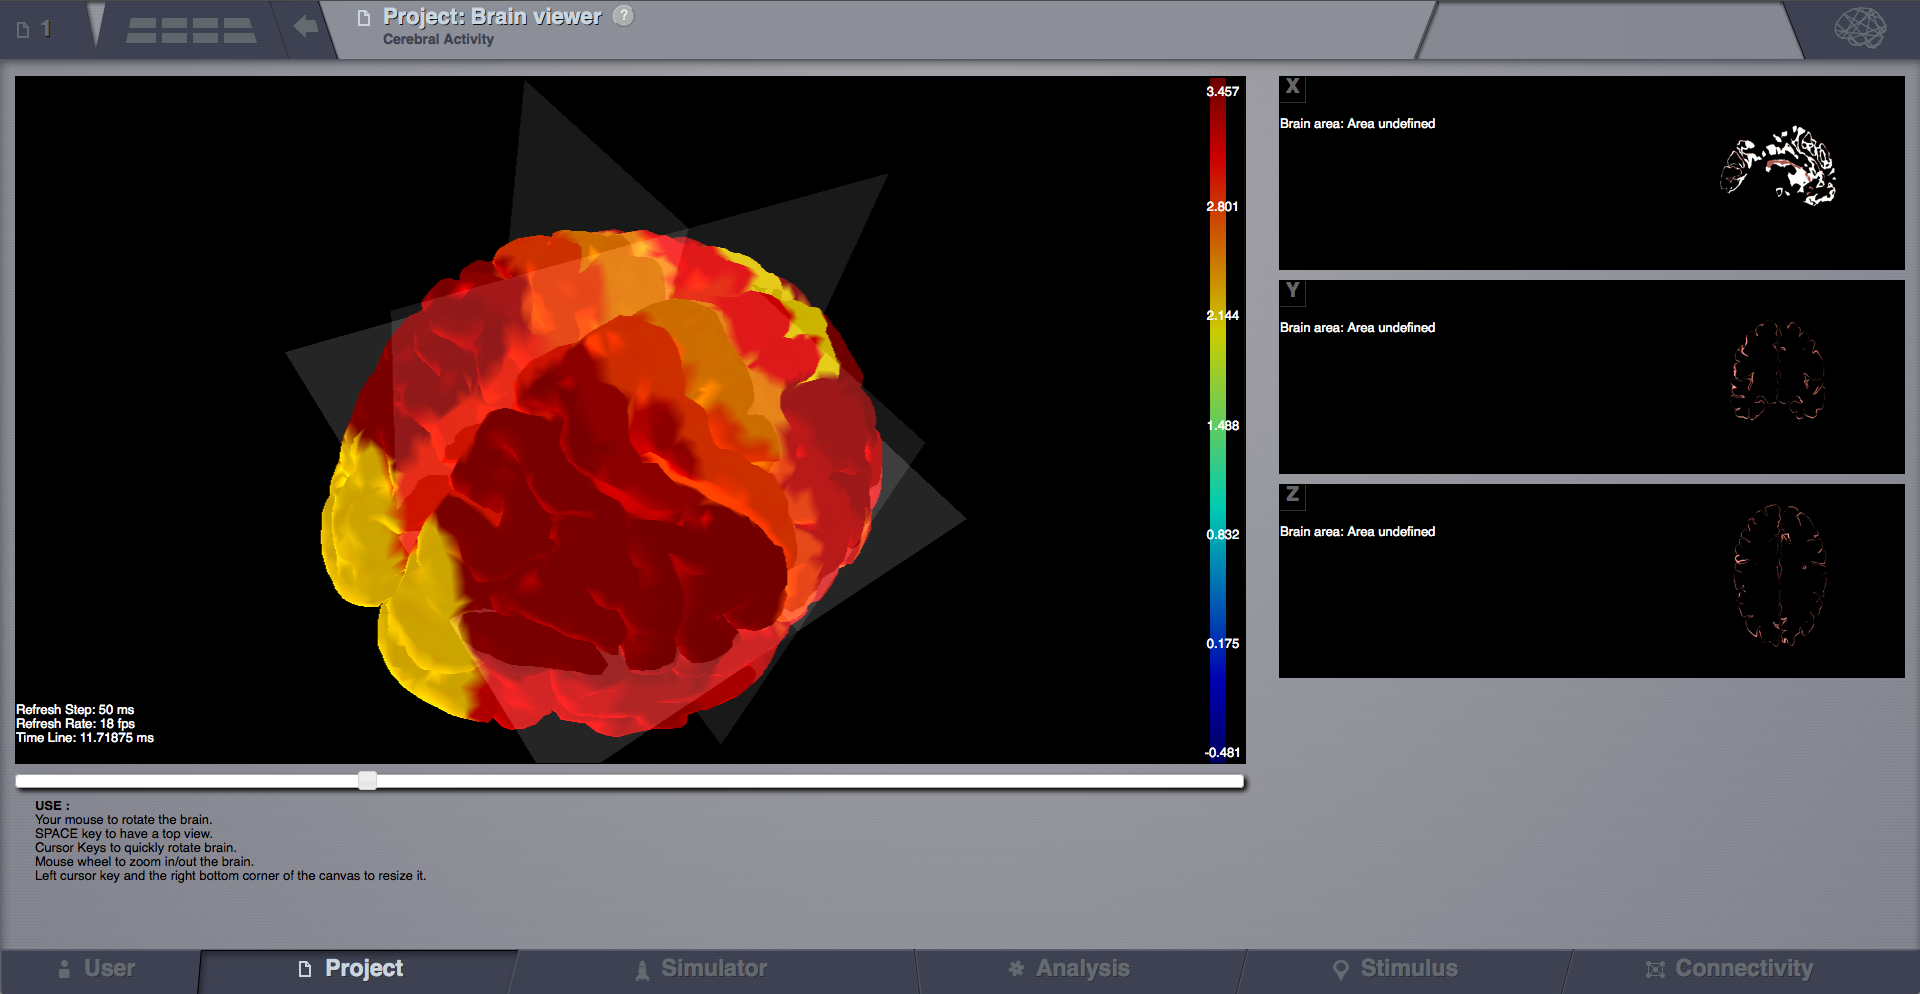
\includegraphics[width=0.48\textwidth]{images/ui_view_brain.png}}
					\\
					\subfloat[][]{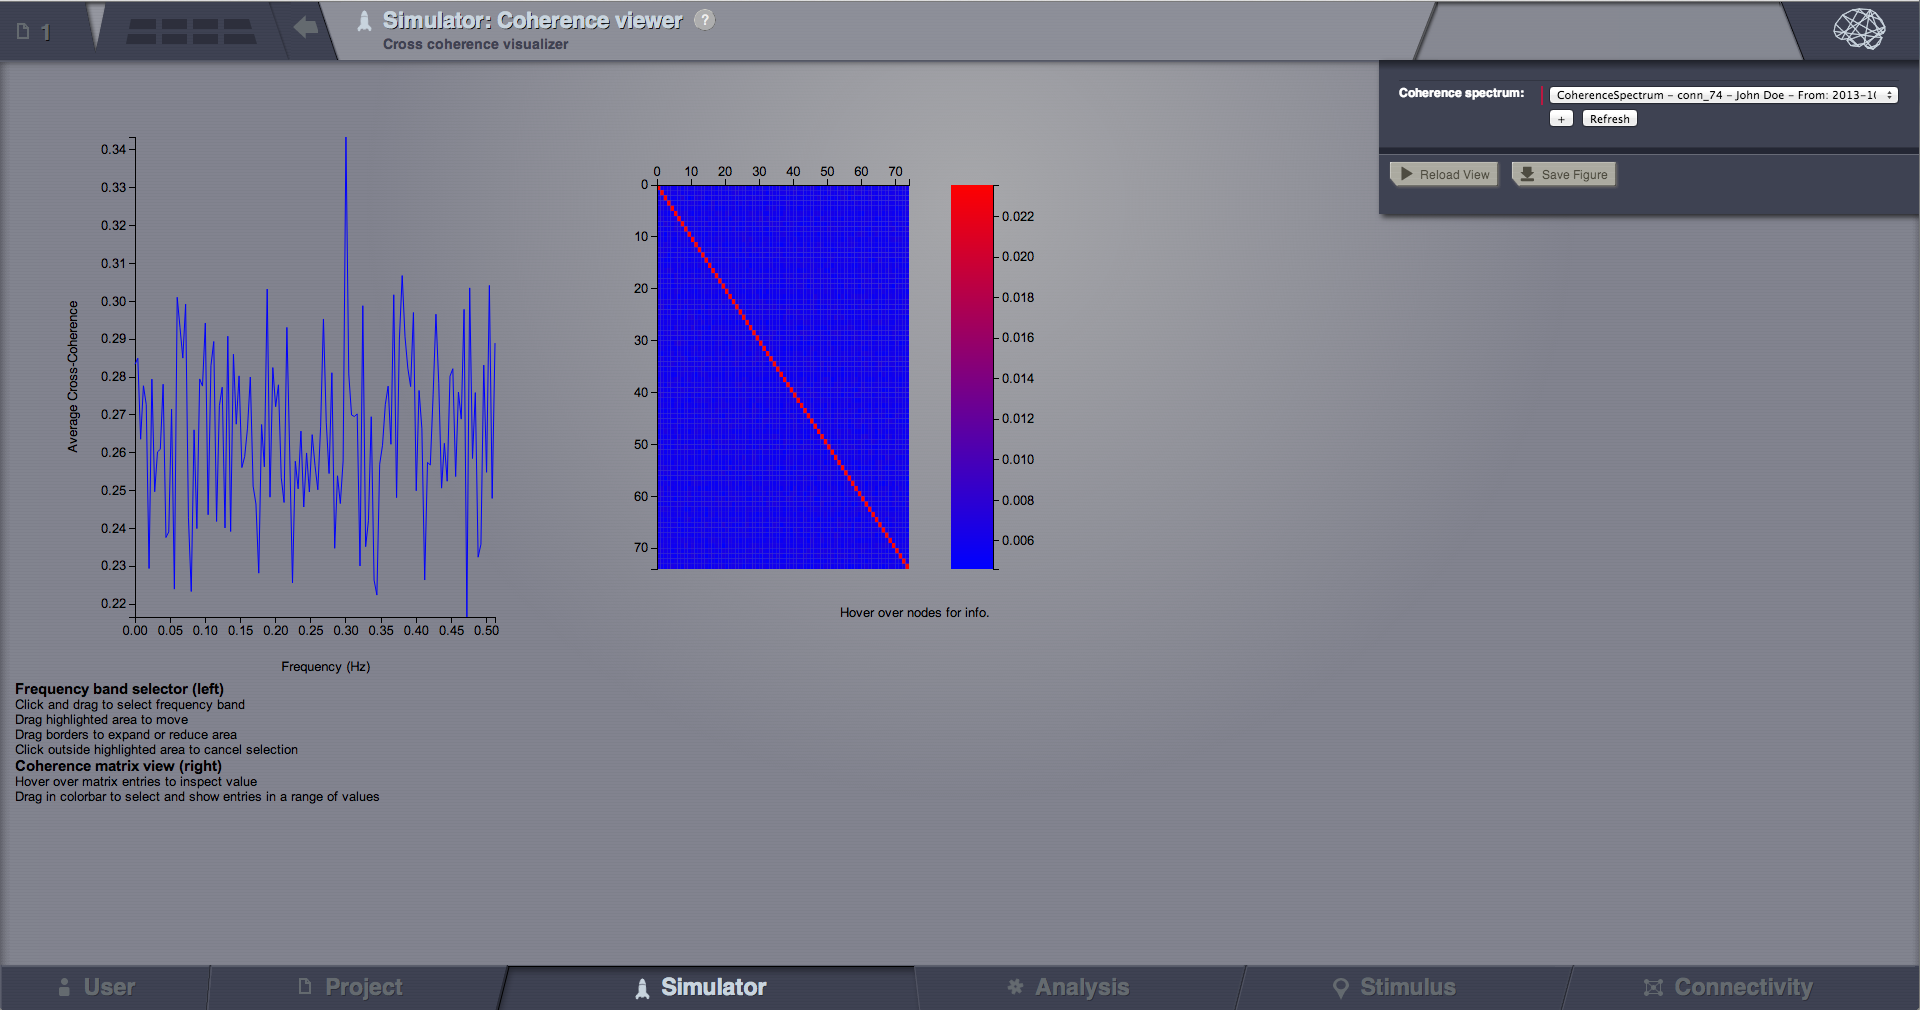
\includegraphics[width=0.48\textwidth]{images/ui_view_coherence.png}}
					\\
					\subfloat[][]{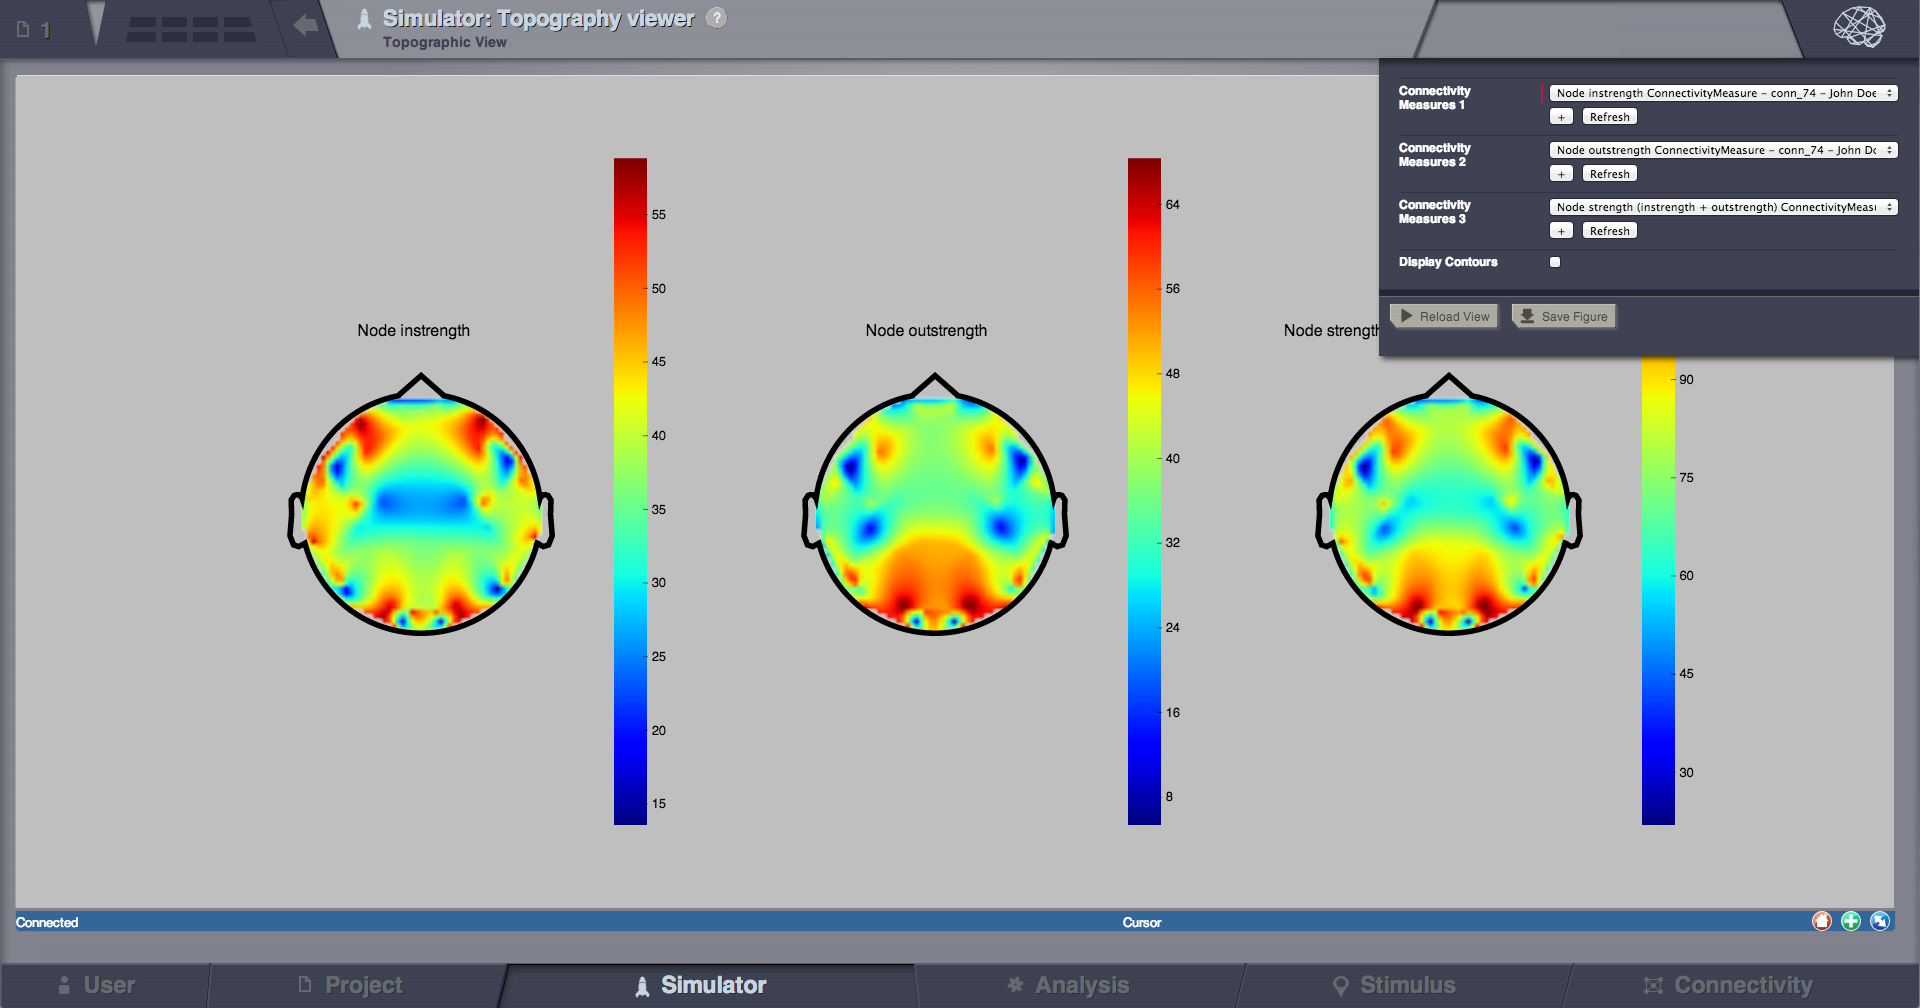
\includegraphics[width=0.48\textwidth]{images/ui_view_topo.png}}
					\\
					\subfloat[][]{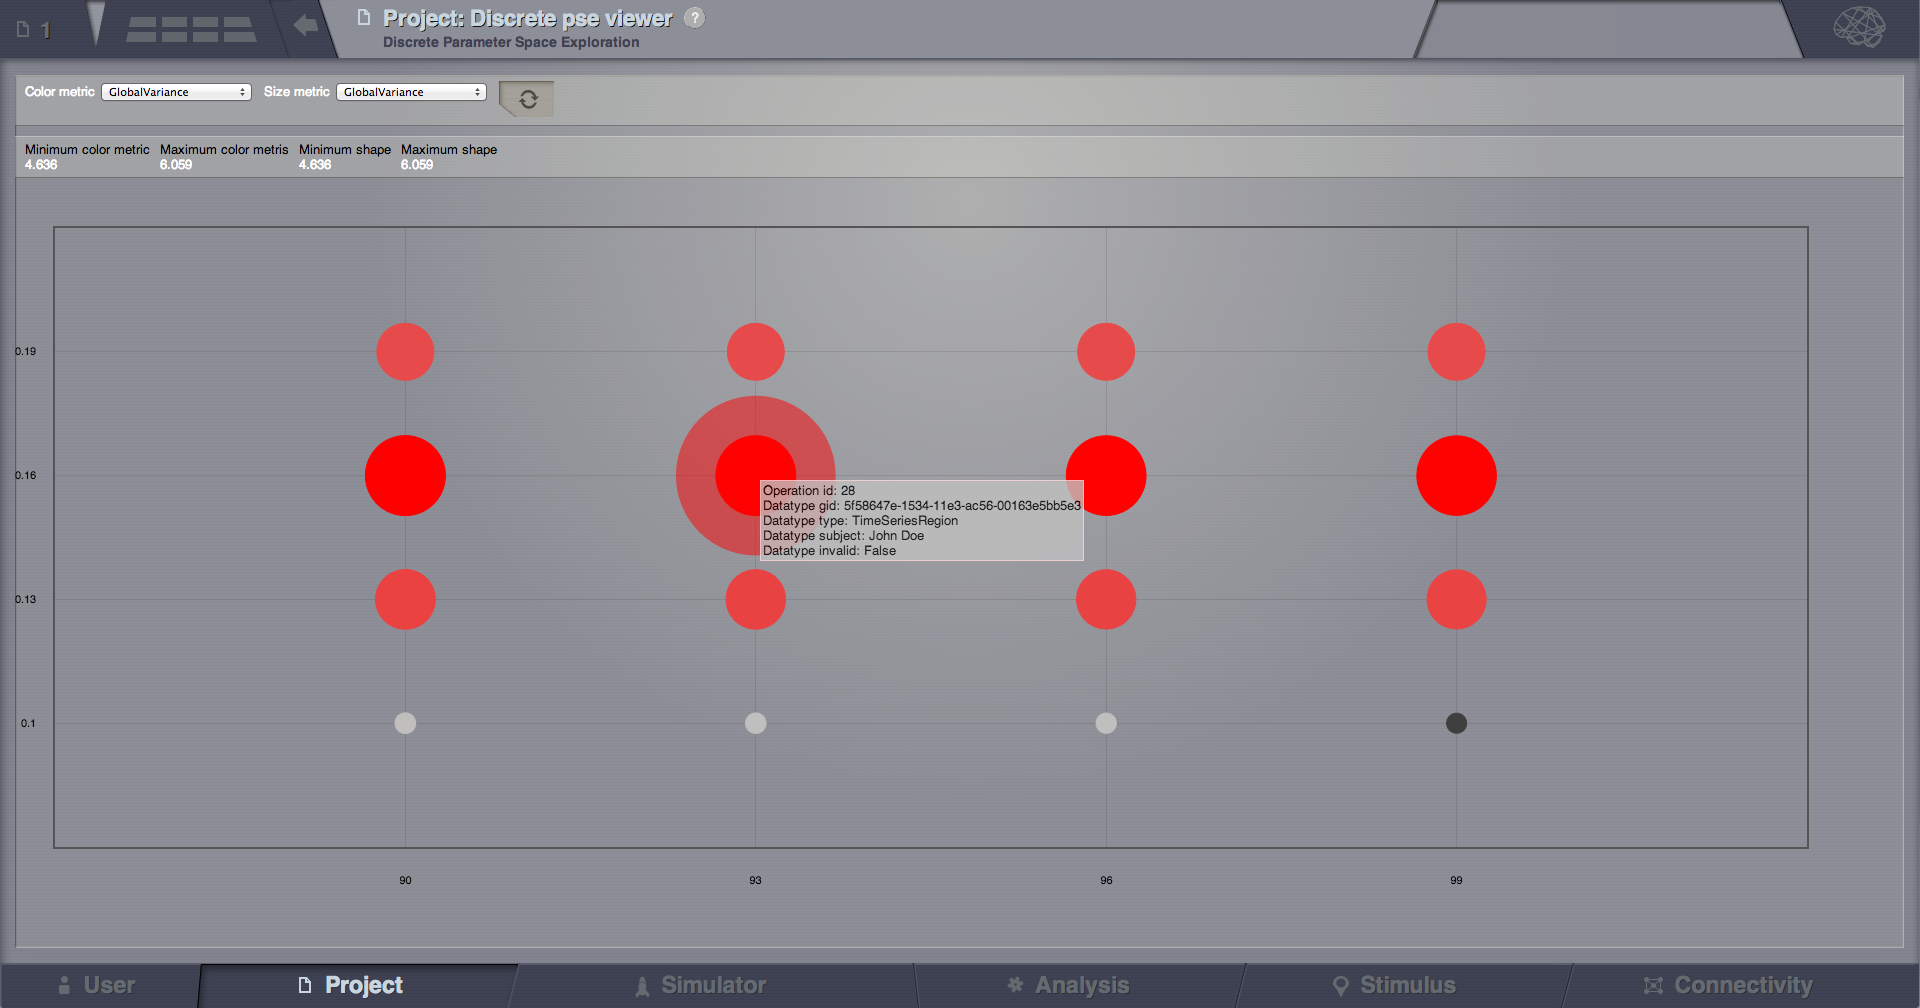
\includegraphics[width=0.48\textwidth]{images/ui_view_pse.png}}
					\caption{\TVB visualizers: 
					(A) WebGL: 3D display of region level simulated signal, mapped on a brain cortical surface
					(B) SVG: Cross Coherence
					(C) MPLH5:  Topographic view with Connectivity in/out strength measures
					(D) FLOT: Parameter Space Exploration results grid}
				\label{fig:visualizers}
			\end{figure}
	
	\begin{enumerate}
		\item \emph{WebGL viewers} are based on \emph{HTML 5 Canvas} element
		and the \emph{GL} context. These viewers offer a 3D display,
		 user interaction with the scene (rotate,
		translate, zoom), and high performance for complex visualizations.
        WebGL is used primarily for visualizing cortical surfaces.
		
		\item \emph{SVG viewers} use a high-quality, highly interactive vectorial 
            format. We
		use such viewers for manipulating and displaying time series,
		covariance or cross coherence datatype results. These visualizers
		were developed specifically for these data types in TVB, and provide a 
		richer level of interaction.

		\item \emph{MPLH5 viewers} use  emph{Matplotlib}'s \emph{HTML 5}
		backend for viewing some of TVB's datatypes, such as
		the Fourier and spectral analyses. 

		\item \emph{Other} simpler viewers in TVB use the JIT
		\url{http://philogb.github.io/jit/} or FLOT
		\url{http://www.flotcharts.org/} Javascript libraries. These are mainly
		2D plots for simple TVB generated data.
	\end{enumerate}

\subsubsection{Connectivity Tools}

		\emph{Connectivity}, in the context of TVB, is another datatype, mapping structural
		information about a subject (a real single individual or an average template). For
		editing and viewing a connectivity, TVB has a dedicated interface, where
		the \emph{G-User} can manipulate connectivity strength and lengths
		at the granularity of individual edges.
        Note that we do not store or use information about the exact anatomical path or
		a connection, only the region centers and connection weights and
		lengths.

 \begin{figure}[!htbp]
		\centering
		\subfloat[][]{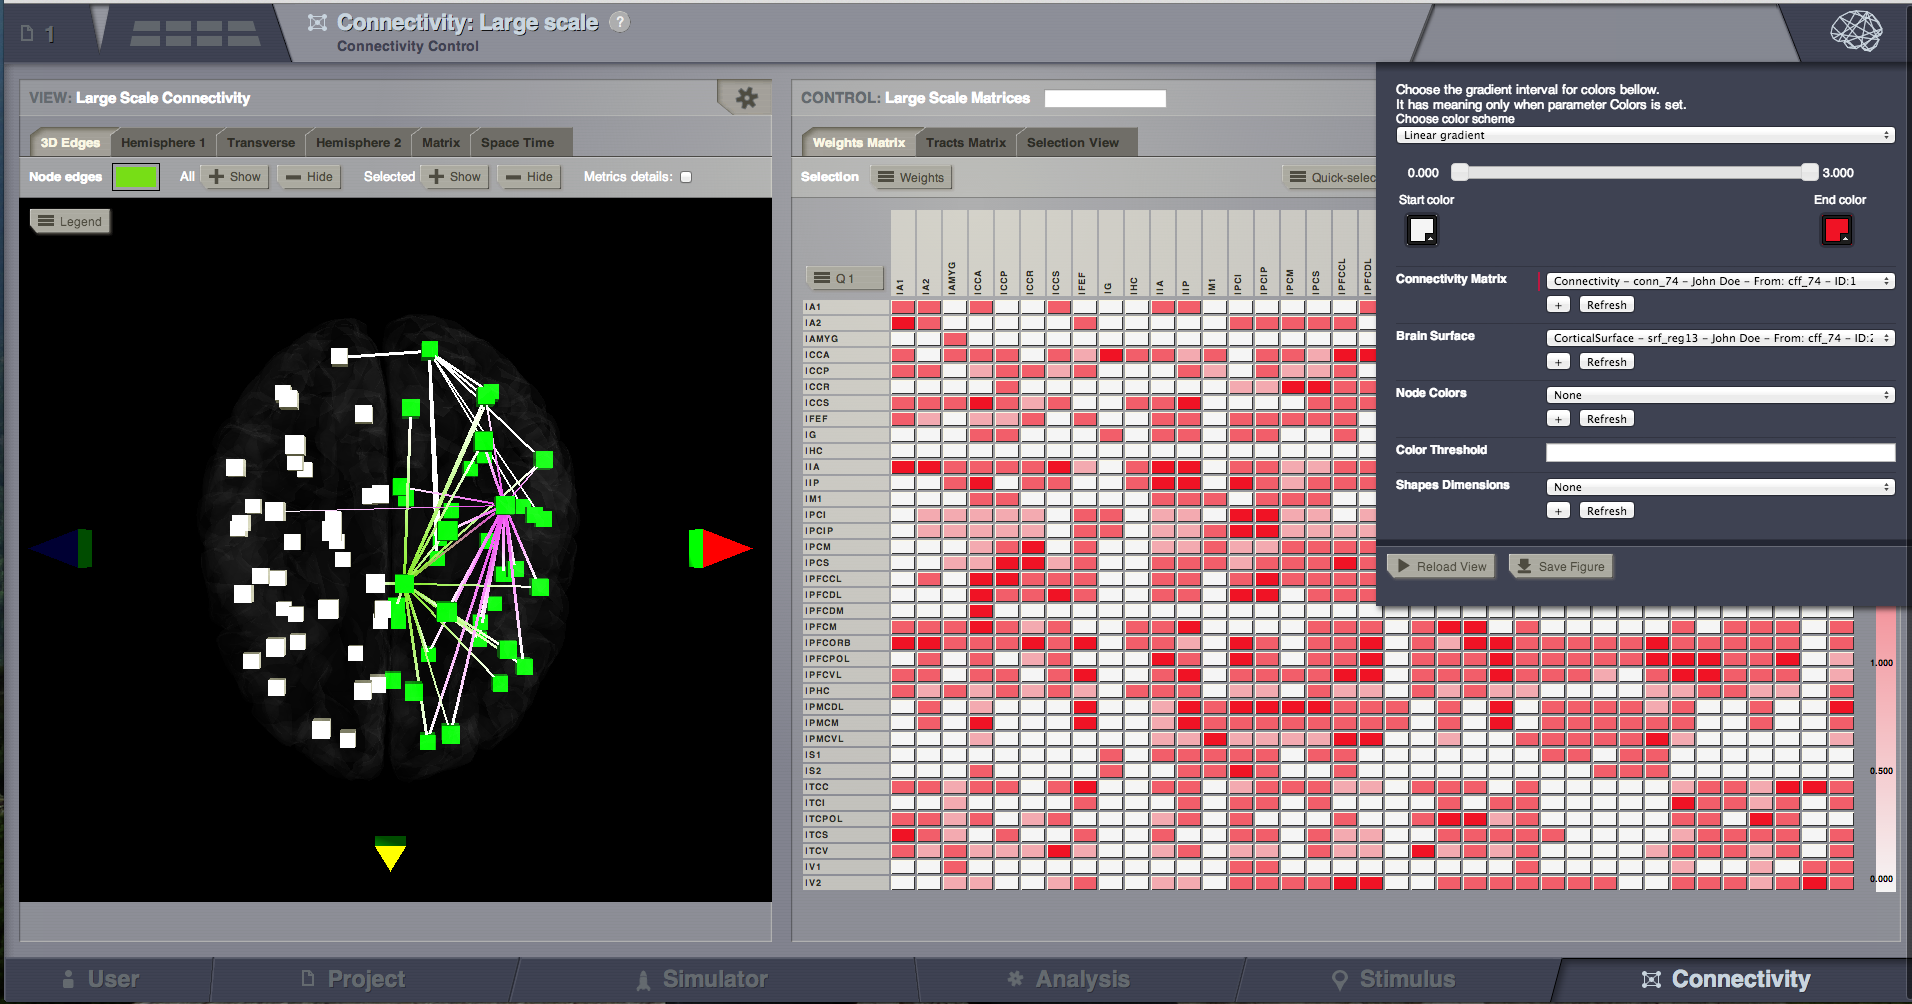
\includegraphics[width=0.48\textwidth]{images/ui_connectivity.png}}
		\\
		\subfloat[][]{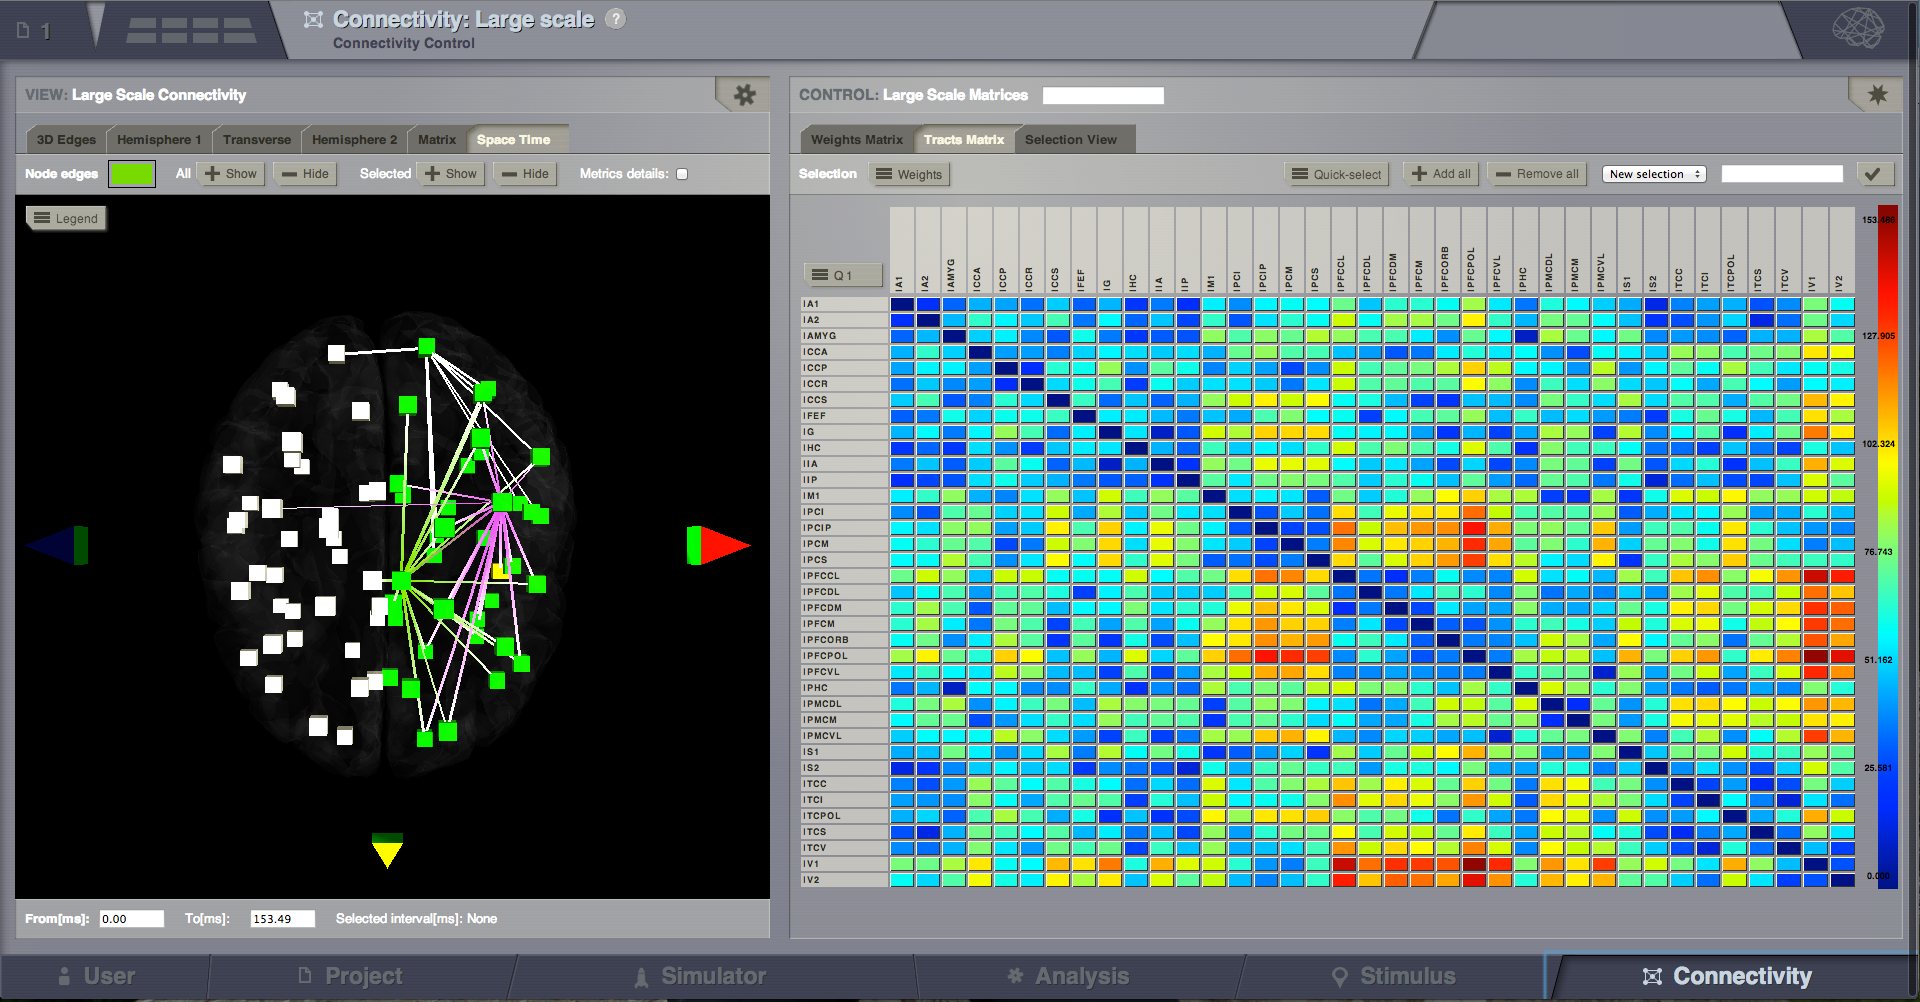
\includegraphics[width=0.48\textwidth]{images/ui_connectivity_delays.png}}
		\caption{Connectivity tools: 
            (A) \textit{Left}: Displaying weighted connections between selection of nodes, with 3D manipulation.
            \textit{Right}: Editing weight connections, one at a time, or many.
            (B) \textit{Left}: Show effect of connectivity delays (in milliseconds) when conduction speed is 1 mm/ms.
        \textit{Right}: Editing and displaying one quadrant from the matrix of connection tracts.}
				\label{fig:connectivity}
\end{figure}

\subsubsection{Stimulus Editor}

    The \emph{Stimulus} interface assists users in generating
	stimulation patterns that maybe be later used in a simulation, for 
    example to model the effects of transcranial magnetic stimulation.
    The way in which stimuli are designed depends on whether the simulation
    will be at region-based or surface-based.
	For region-based simulations, a
	unique temporal profile can be specified for each node, with the amplitude
	of the stimulation modulated individually for each node. For surfaces,
	in addition to the temporal profile, it is possible to select several vertices
	on the surface to define the foci around which the spatial pattern is centered.
    A stimulation profile in TVB is a \emph{pattern}
	datatype, either uniquely temporal or spatiotemporal depending the
	spatial support of the network.

\subsection{Console and scripting}

The components of TVB are of course accessible from a Python
script or, more conveniently, from any of the IPython interfaces.
For example, the tutorials for the simulator have been developed
as IPython notebooks, due to its ability to mix text, mathematics,
code and figures. 

\subsubsection{\texttt{hello\_brain.py}}

To give a basic feel for scripting TVB simulations, we will 
walk through a simple example of a region-level simulation.

\begin{lstlisting}
from tvb.simulator.lab import *
\end{lstlisting}

\noindent which is an all-in-one module making writing scripts
shorter, in the style of \texttt{pylab}, as it imports everything
from \texttt{pylab}, \texttt{numpy} and most of TVB's simulator
modules. Next, we build a simulator object:

\begin{lstlisting}
sim = simulator.Simulator(
    model        = models.Generic2dOscillator(), 
    connectivity = connectivity.Connectivity(),
    coupling     = coupling.Linear(a=1e-2),
    integrator   = integrators.HeunDeterministic(),
    monitors     = (
            monitors.TemporalAverage(), 
    )
)
\end{lstlisting}

\noindent where we've employed a two dimensional oscillator
with default parameters, the default connectivity, a linear 
coupling function with a slope of $1e-2$, and deterministic
Heun integrator and a monitor that temporally averages the 
network dynamics before providing output. Each of these
components can be replaced by a user's subclass of the
appropriate base class, e.g. the value of \texttt{model}
should subclass \texttt{models.Model}.

While TVB strives to keep modules independent of one another,
it is typical for mathematical dependencies to arise between, 
for example, the mass model and the integration time step, so
after configuring a simulator object, it is necessary to invoke

\begin{lstlisting}
sim.configure()
\end{lstlisting}

\noindent which results in walking the tree of objects, checking and 
configuring the constraints among parameters recursively.

The next step is to run through the simulation, collecting
output from the simulator. In this case, it is as simple as

\begin{lstlisting}
ys = array([y for ((t, y),) in  sim(simulation_length=3e2)])
\end{lstlisting}

\noindent where the simulator has been called, returning a 
generator which performs the integration and returns, for each
monitor, the current time and activity. In a case where EEG 
and fMRI monitors, for example, were used, we might write

\begin{lstlisting}
eeg, mri = [], []
for (t_eeg, y_eeg), (t_mri, y_mri) in sim(3e2):
		if y_eeg is not None:
		eeg.append(y_eeg)
		...
\end{lstlisting}

\noindent Because fMRI and EEG monitors have very different
timescales, whenever one monitor return data and the others do
not, the others contain \texttt{None}, hence the check. Building
more complex logic in this loop would permit, for example, online
feedback and modification of connectivity. 

After the simulation loop has finished, you may wish to see the
result, following the previous listing, 

\begin{lstlisting}
plot(ys[:, 0, :, 0], 'k', alpha=0.1)
\end{lstlisting}

\noindent Here we note that \texttt{ys} is four dimensional. The 
simulator has the convention of treating  mass model state as a
three dimensional array of state variables by nodes by statistical
modes. Because \texttt{ys} is an array collected over time, the first
dimension is time, and the plot here is of each node's first state
variable, over time.

Many more demonstrations of the various features of the simulator
can been found in scripts distributed with the sources of TVB, or 
browsed online at \url{https://github.com/the-virtual-brain/scientific_library/tree/trunk/tvb/simulator/demos}.

For more details see the IPython notebook Tutorial: Anatomy of a Region Simulation 
\url{http://nbviewer.ipython.org/urls/raw.github.com/the-virtual-brain
/scientific_library/trunk/tvb/simulator/doc/tutorials/Tutorial_Anatomy
_Of_A_Region_Simulation/Tutorial_Anatomy_Of_A_Region_Simulation.ipynb}

%\subsection{MATLAB Scripting}

%
\subsection{MATLAB Scripting}

Due to the popularity of MATLAB in the neuroscience community, an
interface from MATLAB to \TVB has been introduced that allows a MATLAB
script to design a TVB simulation, run it on TVB and retrieve the 
results. The MATLAB toolbox is provided separately from TVB, at
\url{https://github.com/the-virtual-brain/matlab-tvb}.
In the following, we give a short demonstration and 
describe implementation and rationale.

Because the MATLAB functions need to know the address of the server,
so we take any of the URLs used by the Web UI (here, the one provided
when launching TVB):

\begin{lstlisting}
sv = vb_url('http://127.0.0.1:8080/user/')
\end{lstlisting}

To run simulations without blocking MATLAB, a multiprocessing Pool
is used. We reset the pool and change the number of processes to 6

\begin{lstlisting}
vb_reset(sv, 6)
\end{lstlisting}

Next, we can query the server for information on the classes available,
and also get help for each of the classes

\begin{lstlisting}
info = vb_dir(sv);
\end{lstlisting}

\noindent where info is a cell array of structs, one per module (models,
monitors, etc.) and each struct has a field per class (models.JansenRit, 
models.Kuramoto, etc.). Each of these fields contains the details on 
the class, including all the parameters that can be set. 

To build a simulation, we start with an empty struct
and fill in the details for each part

\begin{lstlisting}
sim = [];

sim.tf = 1e3 % simulation length milliseconds
sim.model.class = vb.models.Generic2dOscillator;
sim.model.a = -2.1;

sim.connectivity.class = 'Connectivity';
sim.connectivity.speed = 4.0;

sim.coupling.class = 'Linear';
sim.coupling.a = 0.002;

sim.integrator.class = 'HeunDeterministic';
sim.integrator.dt = 1e-2;
\end{lstlisting}

Monitors are specified similarly but as a cell array there may be
several of them:

\begin{lstlisting}
sim.monitors{1}.class = 'TemporalAverage';

sim.monitors{2}.class = 'Raw';
sim.monitors{2}.period = 1.0; % ms
\end{lstlisting}

\note[sk]{Raw monitor has no period, or rather the period can't be set as it is
fixed as the integration time step...}

Lastly, we submit the struct as a new simulation

\begin{lstlisting}
[id, data] = vb_new(sv, sim);
\end{lstlisting}

\noindent Lastly, results are returned in a struct, here named data
where each field contians the output of a monitor and can be plotted
and analyzed as a regular MATLAB dataset:

\begin{lstlisting}
plot(data.mon_0_TemporalAverage.ts,...
     squeeze(data.mon_0_TemporalAverage.ys)')
\end{lstlisting}

The implementation of this interface is a combination of an additional
CherryPy controller providing an HTTP/JSON API, running on the same 
server as the Web UI, and a set of MATLAB functions that send HTTP 
GET requests to the server. An implementation based on MEX functions 
invoking the Python library directly was considered, for reasons of 
performance, however, it was judged that such an implementation may be
difficult to stabilize and maintain, given that it would require binary
compatibility between MATLAB, Python and the C compiler. Two additional 
advantages of an HTTP API are that most computational environments have
the ability to connect and make HTTP requests, allowing other programs 
like Perl or Mathematica take advantage of TVB and the approach naturally
extends to work over the network, should TVB be running on another machine.






